\section{Results: from a surrogate library to a fitted ensemble}
\label{sec:results}
\subsection{Different models lead on different datasets}
The library contains strong individual models, but their relative accuracy
depends on the prediction task. Seven of its nine members achieve the lowest
error on at least one PDE dataset. Wavelet transfer leads on Darcy, POD GP on
the Poisson variants, and distribution FNO on the heat variants, while the
ConvNeXt corrector leads on Cavity and Euler. The four additional reaction
diffusion tasks each favor a different library member. This variation motivates keeping
several ways of using coarse information available: choosing one architecture
for the entire collection would discard models that are useful on particular
problems. Table~\ref{tab:allexperts} shows these differences directly, placing
each individual model beside the ensemble rules and the strongest additional
baseline for each dataset.

The best library member outperforms the best available additional baseline on
15 of the 21 PDE datasets. Here the best model in each collection is identified
after evaluation, so this comparison measures the accuracy available within
the library. The fitted mixture also achieves lower aggregate error than the
best additional baseline, while individual baselines remain preferable on
some datasets (Appendix~\ref{app:headlines}). The next question is whether the
reserved fitting examples can turn this available accuracy into a useful
prediction rule. Table~\ref{tab:paperbaselines} summarizes the aggregate
comparisons and Elo ranking, with individual baseline errors in
Appendix~\ref{app:matchedbaselines}.

\begin{table}[t]
\centering\fontsize{7}{8.5}\selectfont\setlength{\tabcolsep}{2.3pt}
\caption{\textbf{Comparing the library, its combinations, and additional baselines.}
All columns report mean relative $L^2$ error in percent on the same evaluation
cases. The best additional baseline is identified by its B label, and M1 to M9
are defined in Table~\ref{tab:paperbaselines}. The selected model uses one member,
the inverse error mixture weights individual errors, and the fitted mixture
optimizes their combination. All three use five fitting examples. Bold marks the lowest unrounded evaluation error.
Daggers mark exclusions in the separate sensitivity analysis
(Appendix~\ref{app:subsets}). Section~\ref{sec:experiments} specifies coverage.
Imported data: Poisson II, Heat II, and Navier Stokes \citep{niu2024}, and ERA5
\citep{hersbach2020,niu2024}.}
\label{tab:allexperts}
\resizebox{\linewidth}{!}{\begin{tabular}{lr|rrrrrrrrr|rrr}
\toprule
Dataset & Best baseline & M1 & M2 & M3 & M4 & M5 & M6 & M7 & M8 & M9 & \shortstack[r]{Selected\\model} & \shortstack[r]{Inverse\\error\\mixture} & \shortstack[r]{Fitted\\mixture} \\
\midrule
Darcy & 3.37 (B1) & 3.07 & 3.44 & 2.78 & 4.98 & \textbf{2.32} & 31.7 & 3.37 & 3.41 & 3.41 & 2.52 & 2.55 & 2.33 \\
Eikonal & 2.21 (B8) & 2.42 & 2.15 & 1.81 & 4.79 & 2.59 & 7.37 & 3.63 & 3.74 & 2.95 & 1.81 & 1.76 & \textbf{1.76} \\
Helmholtz & 4.12 (B9) & \textbf{3.3} & 3.48 & 4.79 & 10.9 & 5.04 & 29.1 & 7.1 & 10.9 & 10.8 & 6.25 & 6.89 & 6.55 \\
Poisson I & \textbf{0.00531} (B2) & 0.0413 & 0.0387 & 0.0427 & 0.0611 & 0.0955 & 9.92 & 0.00684 & 0.128 & 0.0838 & 0.00684 & 0.008 & 0.00788 \\
Poisson II$^{\dagger}$ & 0.0128 (B1) & 0.256 & 0.536 & 0.2 & 25.5 & 0.881 & 26.6 & \textbf{0.0121} & 0.921 & 0.798 & \textbf{0.0121} & 0.0125 & 0.0129 \\
Pressure Poisson$^{\dagger}$ & 0.0639 (B9) & 0.0599 & 0.0695 & 0.0918 & 0.0871 & \textbf{0.0498} & 0.285 & 0.0922 & 0.309 & 0.145 & 0.0734 & 0.0769 & 0.0802 \\
Heat I & 0.0206 (B10) & 0.0164 & 0.0125 & 0.0105 & 0.00915 & 0.0268 & 2.28 & 0.327 & 0.0494 & 0.0149 & 0.00972 & \textbf{0.00593} & 0.0062 \\
Heat II & 0.0201 (B10) & 0.0139 & 0.00878 & 0.00859 & 0.00662 & 0.0173 & 1.58 & 0.312 & 0.0268 & 0.0121 & 0.00662 & 0.00437 & \textbf{0.00435} \\
Cavity & \textbf{0.0419} (B5) & 98.5 & 0.29 & 98.5 & 0.681 & 3.6 & 70.1 & 0.409 & 2.06 & 0.164 & 0.164 & 0.142 & 0.142 \\
Navier Stokes & 1.52 (B10) & 1.55 & 1.69 & 1.57 & 1.58 & 2.33 & 4.41 & 2.79 & 2.62 & 1.95 & 1.61 & 1.52 & \textbf{1.5} \\
Rayleigh Bénard & 0.011 (B10) & 0.0112 & 0.00915 & 0.00715 & 0.00301 & 0.0137 & 0.0999 & 0.295 & 0.0529 & 0.0195 & 0.00301 & 0.00286 & \textbf{0.00269} \\
Burgers & 0.562 (B9) & 0.547 & 0.533 & 100 & 0.507 & 1.28 & 4.88 & 2.5 & 1.69 & 0.545 & 0.516 & 0.513 & \textbf{0.502} \\
Euler & \textbf{5.54} (B2) & 6.2 & 6.08 & 6.72 & 6.3 & 7.43 & 8.13 & 6.15 & 6 & 5.88 & 6.09 & 5.64 & 5.73 \\
Porous medium & 0.0718 (B9) & 0.0448 & 0.0325 & 0.0596 & 0.0654 & 0.126 & 2.75 & 0.909 & 0.681 & 0.0497 & 0.0325 & \textbf{0.0262} & 0.0263 \\
Allen Cahn & 41.2 (B5) & 53 & 52.7 & 42.1 & 45.4 & 41.3 & 102 & 55.5 & 41.4 & 38.8 & 39.4 & 37.9 & \textbf{34.6} \\
Cahn Hilliard I$^{\dagger}$ & 13.3 (B10) & 12.9 & 12.5 & 12.2 & 11.7 & 36.3 & 81.6 & 30.3 & 41.1 & 12.5 & 12.2 & 11.3 & \textbf{10.7} \\
Cahn Hilliard II & 49.8 (B5) & \textbf{46.9} & 48.3 & 51.9 & 50.8 & 60.8 & 99.8 & 64.8 & 55.9 & 47.8 & 52.2 & 47.2 & 49.3 \\
Fisher KPP & 3.24 (B9) & 3.21 & 3.22 & 2.36 & 2.98 & 3.83 & 6.49 & 6.86 & 2.86 & 2.84 & 2.36 & 2.53 & \textbf{2.3} \\
Phase field crystal & 83.5 (B11) & 89.6 & 89.5 & 111 & 83.3 & 202 & 120 & 83.5 & 85.3 & 85.7 & 83.5 & 83.8 & \textbf{83.3} \\
Shallow water & 0.403 (B10) & 0.428 & 0.367 & 0.362 & 0.876 & 0.446 & 1.38 & 1.09 & 1.29 & 0.502 & 0.367 & \textbf{0.357} & 0.389 \\
Wave & \textbf{3.3} (B3) & 6.36 & 6.31 & 4.75 & 11.1 & 5.04 & 64.2 & 24.9 & 8.35 & 11.3 & 4.84 & 4.39 & 4.27 \\
\midrule ERA5 & \textbf{5} (B1) & 14.2 & 17.7 & 20.4 & 12.2 & 9.75 & 9.54 & 6.74 & 20.4 & 8.24 & 6.74 & 5.81 & 6.49 \\
\bottomrule
\end{tabular}
}
\end{table}

\begin{table}[t]
\centering\fontsize{7.5}{9}\selectfont\setlength{\tabcolsep}{3pt}
\caption{\textbf{Model sources and performance, ranked by Elo.}
For each dataset, ratios divide a method's mean evaluation error by the
Selected model's error before geometric averaging. The Selected model is the
member of M1 to M9 with the lowest mean relative $L^2$ error on the five fitting
examples. \textbf{PDE class ratio} averages within each class
and then equally across the seven PDE classes (21 datasets).
\textbf{Dataset ratio} weights all 22 datasets equally, including ERA5.
A ratio of 1 matches selection, 0.90 means 10\% lower aggregate error, and
1.10 means 10\% higher aggregate error. Elo compares each pair of methods on all
22 datasets, with higher ratings better (Appendix~\ref{app:elo}).
M1 to M9 form the library, and B1 to B11
are additional baselines.
Citations identify components or ideas, with adaptations in
Appendix~\ref{app:adaptations}. Individual errors appear in
Table~\ref{tab:allexperts} and Appendix~\ref{app:matchedbaselines}.
Training costs and fine data budgets differ.}
\label{tab:paperbaselines}
\resizebox{\linewidth}{!}{\begin{tabular}{llrrr}
\toprule
Model / rule & Component or idea source & PDE class ratio & Dataset ratio & Elo \\
\midrule
Fitted mixture & \citep{breiman1996} & 0.884 & 0.925 & 1988 \\
Inverse error mixture & \citep{goel2007} & 0.888 & 0.932 & 1951 \\
Selected model & Fitting set selection & 1.000 & 1.000 & 1851 \\
M2 All pairs FNO & \citep{li2021fno,herde2024} & 1.333 & 1.541 & 1688 \\
M1 FiLM FNO transfer & \citep{li2021fno,perez2018} & 1.940 & 2.035 & 1642 \\
M9 ConvNeXt corrector & \citep{liu2022convnext} & 1.695 & 1.867 & 1634 \\
M3 ConvNeXt transfer & \citep{liu2022convnext} & 2.607 & 2.445 & 1619 \\
M4 Distribution FNO & \citep{yu2026fire} & 1.795 & 2.155 & 1592 \\
B10 FNO transfer II & \citep{lyu2023} & 1.794 & 1.850 & 1590 \\
B9 FNO transfer I & \citep{lyu2023} & 1.794 & 1.848 & 1578 \\
M5 Wavelet transfer & \citep{tripura2022wno} & 2.459 & 2.400 & 1528 \\
B5 Latent MF network & \citep{li2022dmfal} & 3.794 & 2.772 & 1497 \\
M7 POD GP & \citep{higdon2008} & 5.492 & 3.108 & 1450 \\
B1 Autoregressive POD GP & \citep{kennedy2000} & 5.854 & 3.362 & 1449 \\
M8 Slice attention corrector & \citep{wu2024transolver} & 4.189 & 3.549 & 1439 \\
B2 Nonlinear POD GP & \citep{perdikaris2017} & 5.871 & 3.626 & 1424 \\
B3 Composite MF MLP & \citep{meng2020} & 4.174 & 3.974 & 1387 \\
B8 Fidelity basis FNO & \citep{li2022ifc} & 8.979 & 6.217 & 1364 \\
B4 Composite MF DeepONet & \citep{howard2023} & 8.001 & 5.803 & 1337 \\
B11 Affine POD GP & \citep{zhang2018} & 17.624 & 11.236 & 1218 \\
B6 Nonlinear decoder transfer & \citep{seidman2022} & 9.927 & 8.252 & 1197 \\
M6 Retrieved field DeepONet & \citep{lu2022mf} & 20.847 & 14.890 & 1057 \\
B7 MFRNP adapter & \citep{niu2024} & 49.969 & 24.194 & 1020 \\
\bottomrule
\end{tabular}
}
\end{table}


\subsection{Combining predictions often improves accuracy}
Using the same five fitting examples, the fitted mixture improves on the
Selected model on 16 of 22 datasets. It reduces geometric mean relative
$L^2$ error by 11.6\% across PDE classes and 7.5\% across all datasets.
Both rules make their decisions before observing the evaluation fields, so
this comparison tests how effectively they use the available fine solutions.
The advantage over a best individual model identified retrospectively from
evaluation answers is much smaller and depends on aggregation
(Appendix~\ref{app:headlines}). The practical benefit is therefore lower error
when model choice must be made before the next fine field is known, with
failures as well as improvements visible in Table~\ref{tab:allexperts}.
Figure~\ref{fig:fieldcomparison} provides one field example.

\begin{figure}[t]
\centering
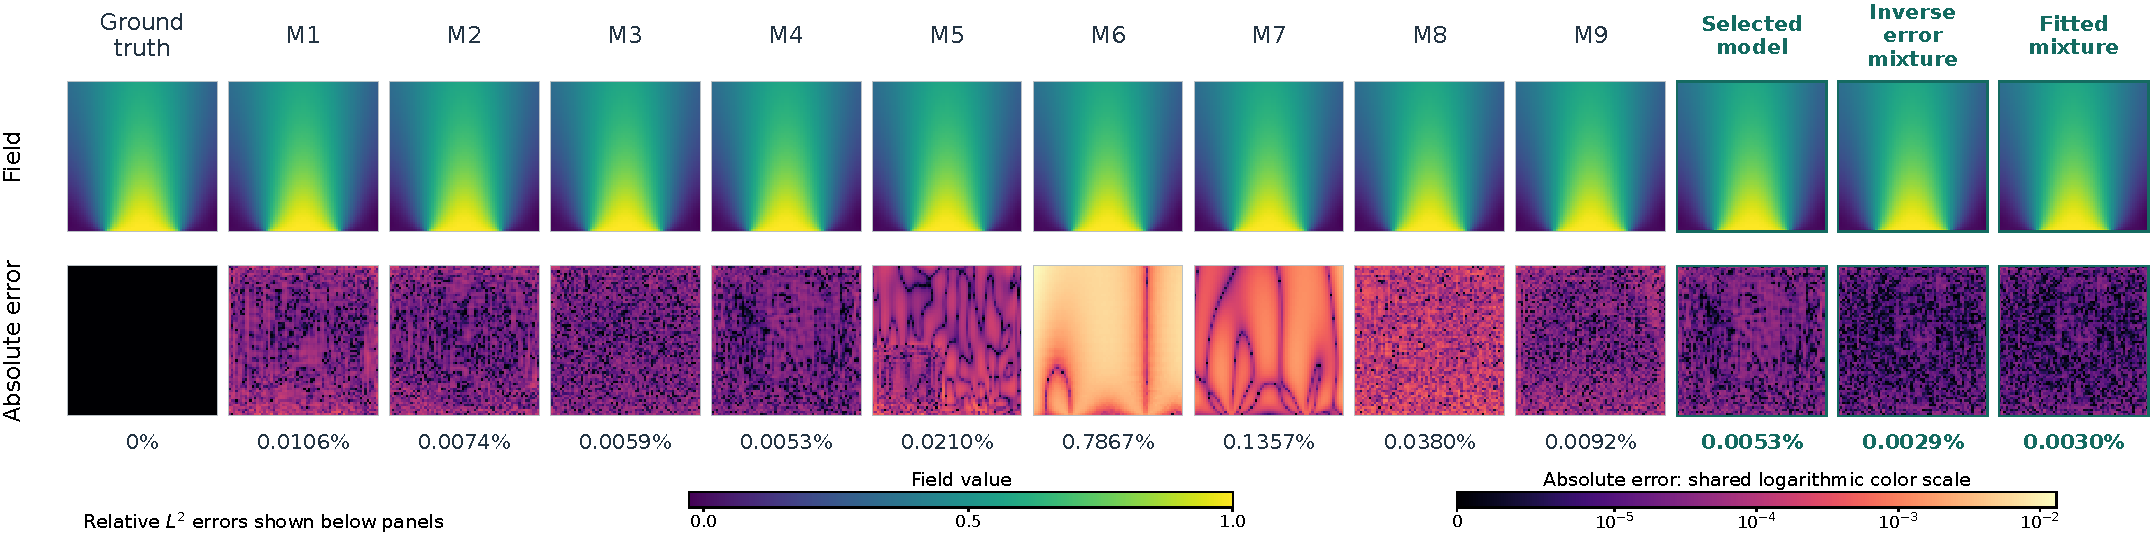
\includegraphics[width=\linewidth]{figures/field_comparison_heat.pdf}
\caption{\textbf{Combining models reduces field error on a Heat I example.}
Top: ground truth, nine model predictions, and the selected model, inverse error
mixture, and fitted mixture.
Bottom: absolute error on a shared logarithmic color scale, with relative $L^2$
error below each panel. Fields share a linear color scale and a $64\times64$ space and time grid.
The three rules use five fitting examples. The selected model is M4 here.
The case is the first evaluation input of the first
partition. The fitted mixture lowers error by 44.4\% relative to the best
individual model.}
\label{fig:fieldcomparison}
\end{figure}

\subsection{Simple weighting captures most of the benefit}
The inverse error mixture nearly matches the fitted mixture in aggregate
accuracy, and the two occupy the highest Elo positions in
Table~\ref{tab:paperbaselines}. Uniform averaging performs poorly
(Table~\ref{tab:main}), indicating that which models receive weight
matters. Yet individual model errors already provide a useful guide to those
weights, with only a small additional gain from joint fitting. The error
analysis supports complementary predictions as a source of improvement
(Appendix~\ref{app:geometry}). Both weighting rules can benefit from that
complementarity, even though the inverse error mixture does not explicitly
estimate interactions between model errors.

\subsection{Sensitivity to fitting and evaluation choices}
The advantage over model selection persists when more fine examples are
available for fitting. Across the 21 PDE datasets, increasing the allowance
from five to twenty examples raises the fitted mixture's reduction in
class aggregated geometric mean relative $L^2$ error from 11.6\% to 13.1\%
(Appendix~\ref{app:budgets}). Both methods receive the same allowance at each
budget, and the surrogate models remain fixed. The modest increase supports
using a small fitting set in these experiments, while leaving the amount
needed for a new problem to be assessed.

Two diagnostics use the same 17 dataset subset to examine dependence on the
evaluation design. Repeating the comparisons on fixed dataset subsets preserves the gain over the Selected
model, while superiority to the best individual model remains sensitive to
the comparison (Appendix~\ref{app:subsets}). We also minimize the reported mean
relative $L^2$ error directly, keeping the trained models and fitting examples
fixed. This gives a modest improvement over fitting squared relative error
(Table~\ref{tab:losscontrol}), identifying the fitting objective as a useful
design choice. This retrospective control is reported separately from the
three main rules.
